\section{IDE Integration}

Apart from improving the language, we have also focused on providing integration with IDEs. This was something new for Flint, as the only existing integration was a Vim and Atom plugin. We chose to integrate Flint with Microsoft Visual Studio Code because it implements the language server protocol, is easy to extend, and is widely used by developers. The details for this feature are listed below:

\begin{itemize}
	\item \#51, \#46 Expose flint compilation API as a “Compiler as a Service”
	\item \#42, \#60 Implement a LSP server
	\item \#61, \#120 Implement LSP server to recompile on file change
	\item \#37 Implement as Flint language extension as a VSCode plugin
\end{itemize}

\subsection{Language Server Protocol}

\begin{figure}[H]
\centering
\makebox[\textwidth]{
\includegraphics[width=\textwidth]{figures/lsp.png}}
\caption{Without LSP, providing language support for Flint requires us to implement fully-featured editor support separately for all editors. With LSP, however, we can support many editors with little overhead.}
\end{figure}

LSP is a protocol which allows a single server implementation for auto-completion, go-to-definition, and diagnostics to be used for multiple editor clients. Unlike implementing a language extension for IDEs such as IntelliJ which would only benefit IntelliJ users, implementing the LSP allows us to provide unified language support across multiple editors. Following our research, we concluded that the best way to integrate Flint with an IDE would be to implement a subset of the Language Server Protocol (LSP). We believe this is the best approach because LSP provides a standardised, documented format for the language support we aim to provide, in addition to being compatible with a range of different editors.

\subsection{Additional Repositories}

We demonstrate our IDE integration with Visual Studio Code as it features the official implementation of a language server client. To do this, we forked the repo owensd/vscode-swift\footnote{\url{https://github.com/owensd/vscode-swift}}, which provides an editor extension that launches the LSP server, describe below.

We also implement a LSP server, which the editor LSP client communicates with to fetch diagnostics, etc. Since Flint is implemented in Swift, the LSP server is implemented in Swift since that avoids implementing any inter-language communication. We base our implementation of the LSP server on theguild/swift-lsp\footnote{\url{https://github.com/theguild/swift-lsp}}, which features a complete definition of the LSP specification. The server runs as a separate target utilising the same modules as the Flint command-line interface, so we have included this in the main repository. The server calls the Flint compiler API, which we refactored to provide a `Compiler as a Service', and communicate with the LSP client using TCP/IP.

\subsection{Implemented Features}

We implement a subset of the LSP server capabilities: display of diagnostics and highlighting the problematic parts of the code.

Given a Flint source file, the compiler returns a list of diagnostics, which can be errors, warnings or notes. Since information about their token positions is collected by the AST passes, the necessary information can be passed to the IDE extension. The IDE then displays all of the messages and highlights the code in question, with a different colour for each diagnostic type. This is illustrated in figure \ref{lsp-use}.

\begin{figure}[H]
\centering
\makebox[\textwidth]{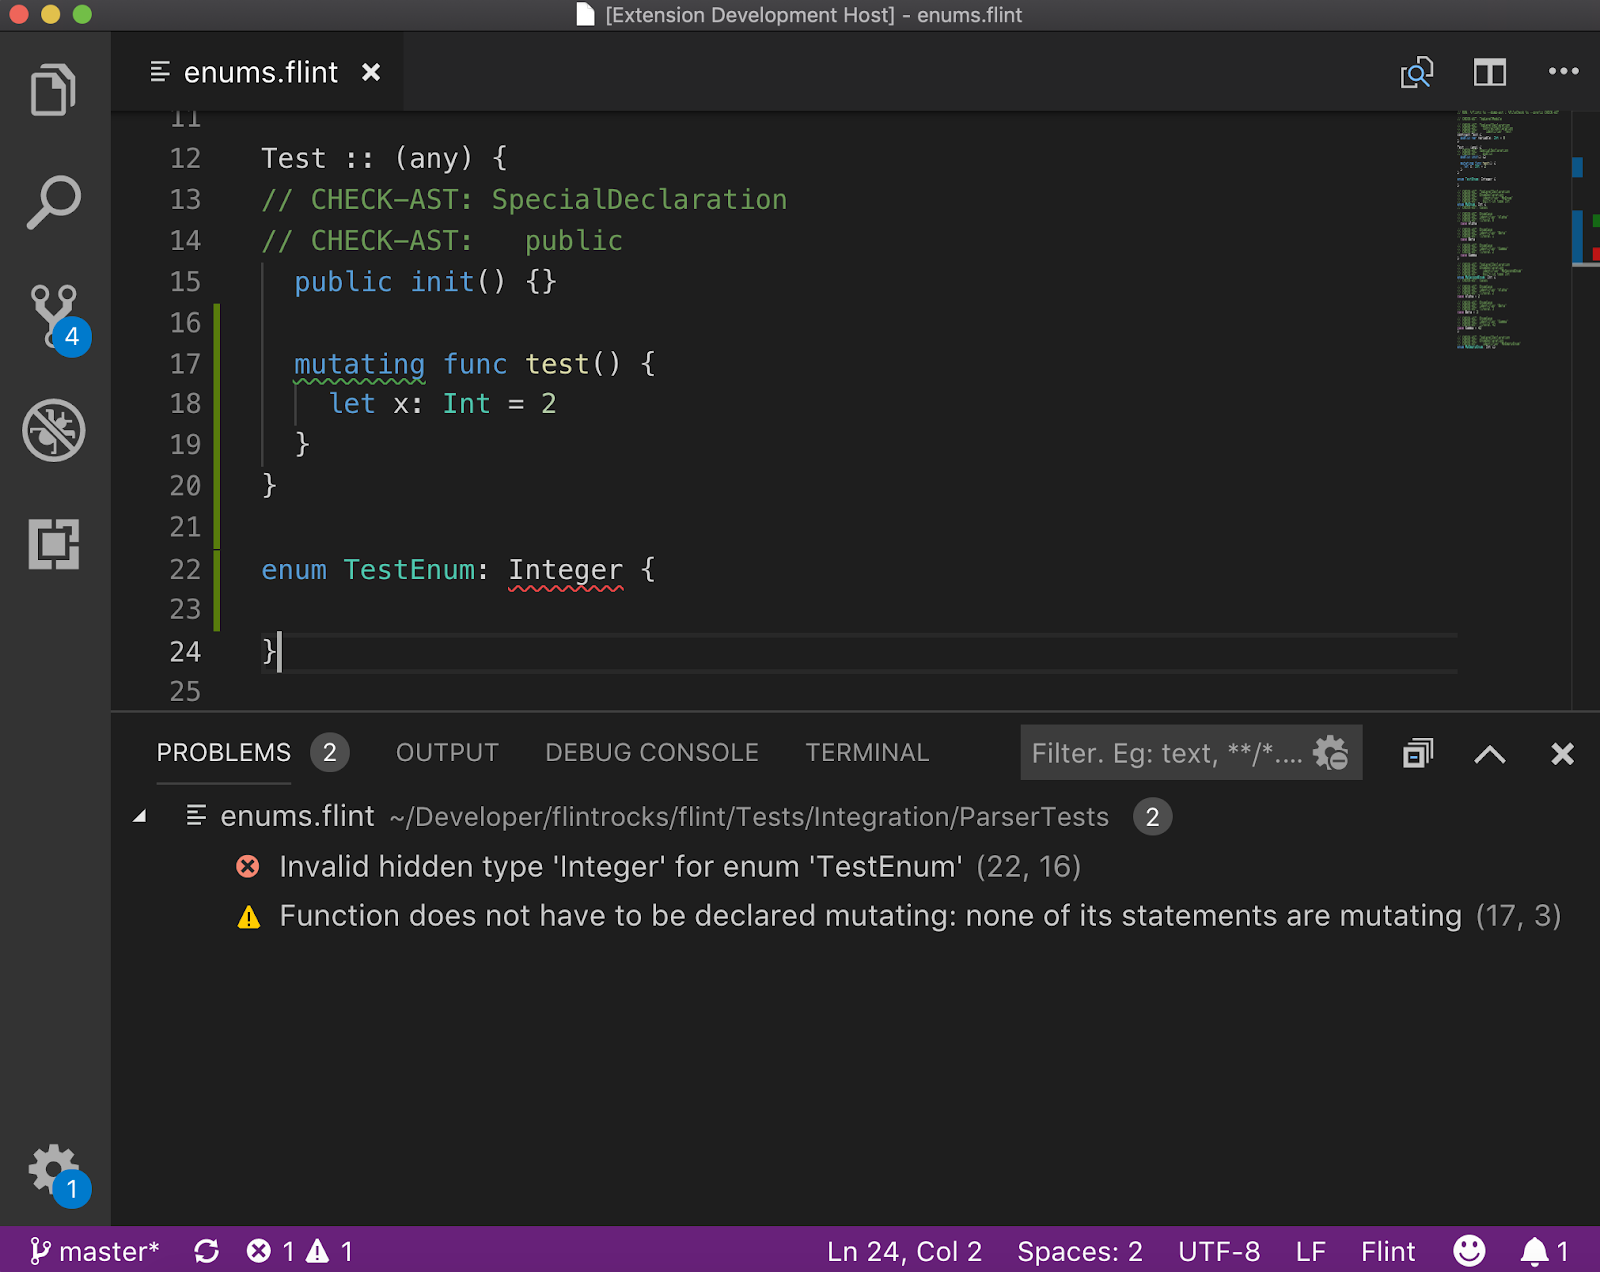
\includegraphics[width=\textwidth]{figures/lsp-use.png}}
\caption{Flint LSP plug-in in use.}
\label{lsp-use}
\end{figure}

The second feature is automatic compilation. This works as expected: once the user stops typing for 2 seconds, the content is automatically compiled and the diagnostics are displayed.

Since every LSP message to the server is processed asynchronously, that allowed us to easily implement the timer by sleeping the thread for 2 seconds and, at the end, check if any new messages were processed in the meantime. That was possible by using global state on the LSP server, which messages can write to. After the thread wakes up from sleeping, if no new messages were processed, that means we can grab the unsaved content from the editor and save it to a temporary location, which we run the Flint compiler on. One important note is that this mechanism does not suffer from concurrency flaws with regards to the shared state and locking is not needed, since messages come through one at a time and will finish sleeping in the same fashion, so we will never have two threads waking up at the same time.

The compiler can run only on files, so saving the content to a file was the easiest option that allowed us to get this working. Another option we considered was to refactor the parser to be highly error-tolerant: the Flint compiler should be able to ingest syntactically incorrect or incomplete Flint code and still generate meaningful ASTs. 

After some exploration of the current parser implementation, we believe that the work involved in making the current parser sufficiently error-tolerant was not viable in the time given. Nevertheless, we note that there are useful articles\footnote{\url{https://github.com/Microsoft/tolerant-php-parser}} on implementing error tolerant parsers used in projects such as Roslyn\footnote{\url{https://github.com/dotnet/roslyn}} and TypeScript\footnote{\url{https://www.typescriptlang.org/}} in the .NET ecosystem, which may be of interest to future Flint maintainers. We thus opted for the first approach as the second approach is much more complicated and does not bring any functional advantages at this stage.
